\documentclass[12pt]{article}
\usepackage[T1, T2A]{fontenc}
\usepackage[utf8]{inputenc}
\usepackage[russian]{babel}
\usepackage{hyperref}
\usepackage{datetime}
\usepackage{amsmath}
\usepackage{amsfonts}
\usepackage{tikz}
\graphicspath{ {./Images/} }

\usepackage{pgfplots}
\usetikzlibrary{calc}
\usetikzlibrary{shapes.geometric}
\pgfplotsset{compat=1.8}

\author{Григорий Матюхин}
\date{\today}
\title{
	Теория вероятностей и математическая статистика \\
	\large Индивидуальное домашнее задание по ТВ и МС \textnumero1.
}

\begin{document}
\maketitle
\newpage
\tableofcontents
\newpage

\section{Выполнение}
\subsection{Задание \textnumero1.}
Найдите вероятность того, что произведение двух последних цифр номера автомобиля:
\begin{enumerate}
	\item Равно 10;
	\item Больше 10;
	\item Меньше 10;
	\item Заключено в промежутке $[15; 45]$.
\end{enumerate}

\subsection*{Решение}
\begin{enumerate}
	\item Равно 10: \\
	      \begin{gather*}
		      \Omega = \{\omega_{ij}; i, j = \overline{0, 9}\}, |\Omega| = 100 \\
		      A = \{\omega_{25}, \omega_{52}\}, |A| = 2 \\
		      P(A) = \frac{|A|}{|\Omega|} \\
		      P(A) = \frac{2}{100} = \frac{1}{50} \\
	      \end{gather*}
	\item Больше 10: \\
	      \begin{gather*}
		      B = \{\omega_{ij}; \omega_{2a}; \omega_{b2}; \omega_{3c}; \omega_{d3}; \} \\
		      i, j, a, b = \overline{4, 9}; a, b = \overline{6, 9}; \\
		      |B| = 56
		      P(B) = \frac{|B|}{|\Omega|} \\
		      P(B) = \frac{56}{100} = \frac{28}{50} \\
	      \end{gather*}
	\item Меньше 10:
	      \begin{gather*}
		      C = \Omega \setminus (A \cup B) \\
		      P(C) = 1 - \frac{1}{50} - \frac{28}{50} \\
		      P(C) = \frac{42}{100} = \frac{21}{50} \\
	      \end{gather*}
	\item Заключено в промежутке $[15; 45]$:
\end{enumerate}

\subsection*{Ответ}

\subsection{Задание \textnumero2.}
В треугольник с вершинами в точках $(a_1;b_1)$, $(a_2;b_2)$ и $(a_3; b_3)$ в соответствии с принципом геометрической вероятности бросается точка.
Обозначим через $\xi$ и $\eta$ координаты этой точки.
Вычислите вероятность того, что квадратное уравнение $x^2 + 2(\xi - c)x + d\eta + f = 0$ будет иметь действительные корни.

\subsection*{Решение}
\subsection*{Ответ}

\subsection{Задание \textnumero3.}
Из двух урн, в каждой из которых находятся $n$ шаров с написанных на них числами от 1 до $n$, наудачу извлекается по одному шару.
Событие $A$ -- сумма чисел, написанных на выбранных шарах, делится на $m$, событие $B$ -- произведение этих чисел больше $k$.
Определите условные вероятности $P(A|B)$ и $P(B|A)$. Являются ли события $A$ и $B$ независимыми?
\subsection*{Решение}
\subsection*{Ответ}

\subsection{Задание \textnumero4.}
Система надежности состоит из 6 элементов и имеет заданную структурную схему. \\
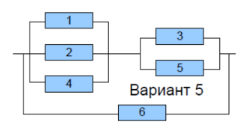
\includegraphics{1.png} \\
События $A_i, i=\overline{1, 6}$, -- отказы элементов за заданный промежуток времени.
\begin{enumerate}
	\item Выразите через события $A_i$ события $A$ и $\overline{A}$, где $A$ — отказ всей системы за заданный промежуток времени.
	\item Считая, что события $A_i$ независимы в совокупности и имеют вероятности $P(A_i)=p_i, i = \overline{1,6}$, вычислите вероятность события $A$.
\end{enumerate}
\subsection*{Решение}
\subsection*{Ответ}

\end{document}
